\documentclass[t, aspectratio=169]{beamer}
\usepackage{amsmath,amsfonts,amsthm,amstext,amssymb, xcolor, tikz, pgf, mathrsfs, polynom, pifont, tabto}

% ----------------------------------------------------------
% Theme Setup

% Use Metropolis Theme
\usetheme[numbering=fraction]{metropolis}
\setbeamertemplate{blocks}[rounded][shadow=false]
\makeatletter
\setlength{\metropolis@titleseparator@linewidth}{1pt}
\makeatother

% Define Colors
\definecolor{chargerblue}{HTML}{002764}
\definecolor{chargerred}{HTML}{e02034}
\definecolor{bggray}{HTML}{d0d3d4}

% Set Colors
\setbeamercolor{title}{fg=chargerblue}
\setbeamercolor{background canvas}{bg=white}
\setbeamercolor{title separator}{fg=chargerred}
\setbeamercolor{structure}{fg=chargerblue}
\setbeamercolor{frametitle}{fg=white, bg=chargerblue}
\setbeamercolor*{normal text}{fg=chargerblue}
\setbeamercolor*{block body}{bg=bggray}
\setbeamercolor*{block title}{bg=chargerblue, fg=white}
% ----------------------------------------------------------

% ----------------------------------------------------------
% Custom Definitions, Commands, Environments, etc.

% Sets of numbers
\def\R{\mathbb{R}} % The reals
\def\N{\mathbb{N}} % The naturals
\def\Z{\mathbb{Z}} % The integers
\def\Q{\mathbb{Q}} % The rationals

% Blank space
\newcommand{\blank}[1]{\underline{\hspace{#1}}} % Blank space

% Change font colors
\newcommand{\cyan}[1]{{\color{cyan}{#1}}} % Changes font to cyan
\newcommand{\red}[1]{{\color{red}{#1}}} % Changes font to red
\newcommand{\magenta}[1]{{\color{magenta}{#1}}} % Changes font to magenta
\newcommand{\orange}[1]{{\color{orange}{#1}}} % Changes font to orange
\newcommand{\yellow}[1]{{\color{yellow}{#1}}} % Changes font to yellow
\newcommand{\violet}[1]{{\color{violet}{#1}}} % Changes font to violet
\newcommand{\green}[1]{{\color{green}{#1}}} % Changes font to green
\newcommand{\blue}[1]{{\color{blue}{#1}}} % Changes font to blue
\newcommand{\white}[1]{{\color{white}{#1}}} % Changes font to white

% Fitted inclusion symbols
\newcommand{\fp}[1]{\left({#1}\right)} % Fitted parentheses around content
\newcommand{\fb}[1]{\left[{#1}\right]} % Fitted brackets
\newcommand{\lhoi}[1]{\left({#1}\right]} % Left half-open interval
\newcommand{\rhoi}[1]{\left[{#1}\right)} % Right half-open interval
\newcommand{\set}[1]{\left\{{#1}\right\}} % Fitted braces (useful for sets)
\newcommand{\av}[1]{\left|{#1}\right|} % Fitted absolute value bars

% Augmented Matrix Environment
\newenvironment{amatrix}[1]{%
	\left[\begin{array}{@{}*{#1}{c}|c@{}}
	}{%
	\end{array}\right]
}

% Miscellaneous
\def\then{\Rightarrow}
\def\to{\rightarrow}
\def\d{^{\circ}}
\newcommand{\?}{\stackrel{?}{=}}
\newcommand{\cmark}{\text{ \ding{51}}}
\newcommand{\xmark}{\text{ \ding{55}}}

% Coordinate Plane (Four-Quadrant)
\def\coordplane {
	\begin{tikzpicture}        \draw[step=0.25cm,black,very thin,opacity=0.25] (-2.5cm, -2.5cm) grid (2.5cm, 2.5cm);
		\draw[<->,thick,black] (-2.5cm, 0) -- (2.5cm, 0) node[anchor=north west,pos=0.94,font=\scriptsize]{$x$};
		\draw[<->,thick,black] (0,-2.5cm) -- (0, 2.5cm) node[anchor=south east,font=\scriptsize,pos=0.94]{$y$};
	\end{tikzpicture}
}

% Coordinate Plane (One-Quadrant)
\def\onequad {
	\begin{tikzpicture}
		\draw[step=0.25cm, black, very thin, opacity=0.25] (0,0) grid (7.5cm,5cm);
		\draw[->, thick, black] (0,0) -- (7.5cm, 0) node[anchor=north west,font=\scriptsize,pos=0.94]{$x$};
		\draw[->, black, thick] (0,0) -- (0,5cm) node[anchor=south east,font=\scriptsize,pos=0.94]{$y$};
	\end{tikzpicture}
}
% ----------------------------------------------------------

% ----------------------------------------------------------
% Presentation Information
\title[VL3]{Organizing Data; Histograms, Frequency Polygons, and Ogives}
\subtitle{2-1 and 2-2}
\author{Jacob Ayers}
\institute{Lesson \#3}
\date{MAT 110}
% ----------------------------------------------------------

\begin{document}
	
	% Slide 1 (Title Slide)
	\begin{frame}
		\titlepage
	\end{frame}
	
	% Slide 2 (Objectives)
	\begin{frame}{Objectives}
		\begin{itemize}
			\item Organize data using categorical frequency distributions, ungrouped frequency distributions, and grouped frequency distributions
			\item Find class width, boundaries, and midpoints for grouped data
			\item Use histograms, frequency polygons, and ogives to visualize frequency distributions
		\end{itemize}
	\end{frame}

	\begin{frame}{Organizing Data}
		Last week, you learned how researchers gather data. \pause
		
		Now, we'll turn our attention to organizing that data. \pause
		
		\begin{block}{Definition}
			A \textit{frequency distribution} is the organization of raw data in table form, using classes and frequencies.
		\end{block} \pause
	
		When creating a frequency distribution, we divide the data into categories (classes) and then determine how many data values fall into each category (frequencies).
	\end{frame}

	\begin{frame}{Categorical Frequency Distributions}
		When data can be placed into qualitative categories, we use categorical frequency distibutions. \pause
		
		Examples: \begin{itemize}
			\item blood type
			\item political party
			\item college major
		\end{itemize} \pause
	
		To make the frequency distribution, tally how many data values are in each category and list it in table form. We can also determine relative frequencies, using percentages. 
	\end{frame}

	\begin{frame}{Categorical Frequency Distributions}
		Twenty-five army inductees were given a blood test to determine their blood type. The data set is below. Construct a categorical frequency distribution for the data. \pause
		
		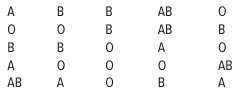
\includegraphics[width=1.5in]{blood-types.png} \pause
		
		\begin{tabular}{c|c|c}
			Blood Type & Frequency & Percent \\ \hline
			A & 5 & $5 \div 25 = 20\%$ \\
			B & 7 & $7 \div 25 = 28\%$ \\
			O & 9 & $9 \div 25 = 36\%$ \\
			AB & 4 & $4 \div 25 = 16\%$ \\ \hline
			TOTALS & 25 & 100\%
		\end{tabular}
	\end{frame}

	\begin{frame}{Ungrouped Frequency Distributions}
		When dealing with numerical data that is all in a small range, an ungrouped frequency distribution can be used. \pause
		
		An ungrouped frequency distribution is just a categorical distribution where the categories are quantitative rather than qualitative. \pause
		
		Example: The ages of 20 dogs in a pet shelter are shown. Construct an ungrouped frequency distribution for the data. \pause
		
		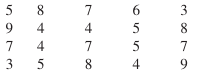
\includegraphics[width=1.5in]{dog-ages.png} \pause
		
		Since there are only 7 unique ages, it makes sense to use an ungrouped distribution here.
	\end{frame}

	\begin{frame}{Ungrouped Frequency Distributions}
		Here is the ungrouped frequency distribution:
		
		\begin{tabular}{c|c}
			Age & Frequency \\ \hline
			3 & 2 \\
			4 & 4 \\
			5 & 4 \\
			6 & 1 \\
			7 & 4 \\
			8 & 3 \\
			9 & 2
		\end{tabular}
	\end{frame}

	\begin{frame}{Grouped Frequency Distributions}
		When data values are spread over a large range, it doesn't make sense to have individual classes for each value. We must group data into wider classes. \pause
		
		Below is an example of a grouped frequency distribution:
		
		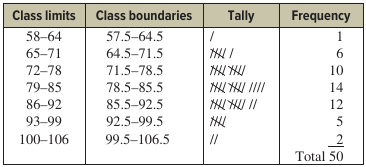
\includegraphics[width=3in]{sample-gfd.png}	
	\end{frame}

	\begin{frame}{Grouped Frequency Distributions}
		Here is the first row again: \pause
		
		\begin{tabular}{|c|c|c|}
			\hline Class limits & Class boundaries & Frequency \\ \hline
			58-64 & 57.5-64.5 & 1 \\ \hline
		\end{tabular} \pause
	
		Some things to note: \begin{itemize} \vspace{-12pt}
			\item 58 = lower class limit - smallest data value in the class \pause
			\item 64 = upper class limit - largest data value in the class \pause
			\item Class boundaries - eliminate gaps in the distribution \pause
			\item Class width = (Lower Limit) - (Lower Limit) (in this case, 65 - 58 = 7)
		\end{itemize}
	\end{frame}

	\begin{frame}{Grouped Frequency Distributions}
		Some rules to follow when constructing a grouped frequency distribution: \begin{itemize} \vspace{-12pt} \pause
			\item Use 5-20 classes \pause
			\item Preferably, use odd class width (ensures midpoints are same place value as data) \pause
			\item Classes must be \textit{mutually exclusive} (i.e. no overlap) \pause
			\item Classes must be \textit{continuous} (i.e. no gaps) \pause
			\item Classes must be \textit{exhaustive} (i.e. all data values must be in a class) \pause
			\item Classes must be equal in width
		\end{itemize}
	\end{frame}

	\begin{frame}{Grouped Frequency Distributions}
		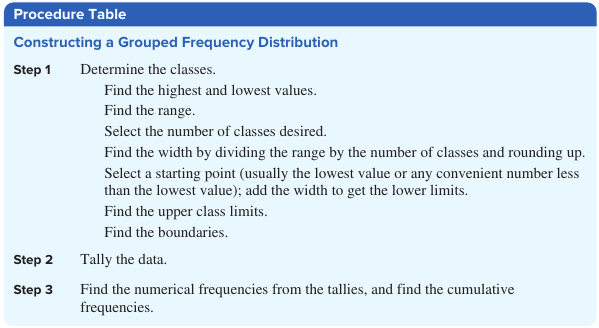
\includegraphics[width=5in]{gfd-procedure.png}
	\end{frame}

	\begin{frame}{Grouped Frequency Distributions}
		The number of stories in each of a sample of the world's 30 tallest buildings follows. Construct a grouped frequency distribution with 7 classes.
		
		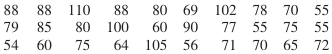
\includegraphics[width=3in]{building-data.png} \pause
		
		\underline{Step 1: Determine the Classes} \\
		Highest Value: 110; Lowest Values: 54 \pause \\
		Range = 110 - 54 = 56 \pause \\
		Class width = $56 \div 7 = 8$; round up to next odd number: $9$ \pause \\
		Starting point: 54
	\end{frame}

	\begin{frame}{Grouped Frequency Distributions}
		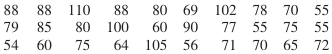
\includegraphics[width=3in]{building-data.png}
		
		\underline{Steps 2 and 3: Tally Data; Find Numerical Frequencies} \\
		\begin{tabular}{|c|c|p{3cm}|c|} \hline
			Class Limits & Class Boundaries & Tally & Frequency \\ \hline
			54-62 & \onslide<2->{53.5-62.5} &  & \onslide<3->{7} \\ \hline
			63-71 & \onslide<2->{62.5-71.5} &  & \onslide<3->{6} \\ \hline
			72-80 & \onslide<2->{71.5-80.5} &  & \onslide<3->{8} \\ \hline
			81-89 & \onslide<2->{80.5-89.5} &  & \onslide<3->{4} \\ \hline
			90-98 & \onslide<2->{89.5-98.5} &  & \onslide<3->{1} \\ \hline
			99-107 & \onslide<2->{98.5-107.5} &  & \onslide<3->{3} \\ \hline
			108-116 & \onslide<2->{107.5-116.5} &  & \onslide<3->{1} \\ \hline
		\end{tabular}
	\end{frame}

	\begin{frame}{Histograms, Frequency Polygons, and Ogives}
		Once data has been organized, it is often helpful to display it visually. \pause
		
		The three most common graphs in research are: \begin{itemize}
			\item Histograms
			\item Frequency Polygons
			\item Ogives
		\end{itemize} \pause
	
		We will go over each graph in turn.
	\end{frame}

	\begin{frame}{Histograms, Frequency Polygons, and Ogives}
		Below is the procedure for constructing these three graphs. \pause
		
		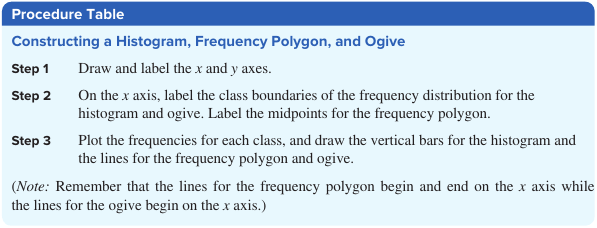
\includegraphics[width=5in]{graphs-procedures.png} \pause
		
		We will use Google Sheets to construct these graphs.
	\end{frame}

	\begin{frame}{Histograms}
		Histogram: displays data using vertical bars \pause
		
		Construct a histogram for the following data:
		
		\begin{tabular}{|c|c|} \hline
			Class boundaries & Frequency \\ \hline
			99.5-104.5 & 2 \\
			104.5-109.5 & 8 \\
			109.5-114.5 & 18 \\
			114.5-119.5 & 13 \\
			119.5-124.5 & 7 \\
			124.5-129.5 & 1 \\
			129.5-134.5 & 1 \\ \hline
		\end{tabular}
	\end{frame}

	\begin{frame}{Frequency Polygons}
		Frequency Polygon: displays data using lines that connect points plotted for frequencies at midpoints of classes \pause
		
		Construct a frequency polygon for the following data:
		
		\begin{tabular}{|c|c|c|} \hline
			Class boundaries & Midpoints & Frequency \\ \hline
			99.5-104.5 &  & 2 \\
			104.5-109.5 &  & 8 \\
			109.5-114.5 &  & 18 \\
			114.5-119.5 &  & 13 \\
			119.5-124.5 &  & 7 \\
			124.5-129.5 &  & 1 \\
			129.5-134.5 &  & 1 \\ \hline
		\end{tabular}
	\end{frame}

	\begin{frame}{Ogives}
		Ogive: line graph that represents cumulative frequencies for each class \pause
		
		Construct an ogive for the following data:
		
		\begin{columns}
			\begin{column}{0.5\textwidth}
				\begin{tabular}{|c|c|} \hline
					Class boundaries & Frequency \\ \hline
					99.5-104.5 & 2 \\
					104.5-109.5 & 8 \\
					109.5-114.5 & 18 \\
					114.5-119.5 & 13 \\
					119.5-124.5 & 7 \\
					124.5-129.5 & 1 \\
					129.5-134.5 & 1 \\ \hline
				\end{tabular}
			\end{column}
			\begin{column}{0.5\textwidth}
				\begin{tabular}{|c|c|} \hline
					 & Cumulative Frequency \\ \hline
					Less than 99.5 & 0 \\
					Less than 104.5 & 2 \\
					Less than 109.5 & 10 \\
					Less than 114.5 & 28 \\
					Less than 119.5 & 41 \\
					Less than 124.5 & 48 \\
					Less than 129.5 & 49 \\
					Less than 134.5 & 50 \\ \hline
				\end{tabular}
			\end{column}
		\end{columns}
	\end{frame}

	\begin{frame}{Putting It Together}
		The number of faculty listed
		for a sample of private colleges that offer only bachelor’s
		degrees is listed below. Use these data to construct a fre­quency distribution with 7 classes, a histogram, a frequency
		polygon, and an ogive. \pause
		
		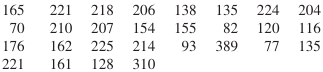
\includegraphics[width=3in]{faculty-data.png}
		
		\underline{Step 1: Determine the Classes} \\
		Highest: 389; Lowest: 70 \pause \\
		Range: 389 - 70 = 329 \pause \\
		Class width = $329 \div 7 = 47$ \pause \\
		Starting point: 70
	\end{frame}

	\begin{frame}{Putting It Together}
		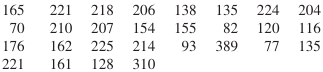
\includegraphics[width=3in]{faculty-data.png}
		
		\underline{Steps 2 and 3: Tally Data; Find Numerical Frequencies} \\
		\begin{tabular}{|c|c|c|p{3cm}|c|} \hline
			Class Limits & Class Boundaries & Class Midpoints & Tally & Frequency \\ \hline
			70-116 & \onslide<2->{69.5-116.5} & \onslide<3->{93} &  & \onslide<4->{5} \\ \hline
			117-163 & \onslide<2->{116.5-163.5} & \onslide<3->{140} &  & \onslide<4->{9} \\ \hline
			164-210 & \onslide<2->{163.5-210.5} & \onslide<3->{187} &  & \onslide<4->{6} \\ \hline
			211-257 & \onslide<2->{210.5-257.5} & \onslide<3->{234} &  & \onslide<4->{6} \\ \hline
			258-304 & \onslide<2->{257.5-304.5} & \onslide<3->{281} &  & \onslide<4->{0} \\ \hline
			305-351 & \onslide<2->{304.5-351.5} & \onslide<3->{328} &  & \onslide<4->{1} \\ \hline
			352-398 & \onslide<2->{351.5-398.5} & \onslide<3->{375} &  & \onslide<4->{1} \\ \hline
		\end{tabular}
	\end{frame}

	\begin{frame}{Next Steps}
		\begin{itemize}
			\item Read 2-3
			\item Watch Video Lesson \#4
			\item Complete Assignment 2
		\end{itemize}
	
		\vfill
		
		Thanks for watching!
	\end{frame}
	
\end{document}